% Chapter 2

\chapter{Background} % Main chapter title

\label{Background} % For referencing the chapter elsewhere, use \ref{Chapter1} 

\lhead{Chapter 2. \emph{Background}} % This is for the header on each page - perhaps a shortened title

This chapter gives an overview of the state-of-the-art methods in evolutionary algorithms. It gives an in-depth discussion about the intersection of evolutionary algorithms and robotics. This discussion focuses mostly on how evolutionary methods are used to evolve robot designs and controllers for some applications. In addition, genetic algorithms, the role of the encoding in the representation within an evolutionary setting,  how artificial neural networks (ANNs) can represent an organism in evolutionary algorithms (EAs), and how these ANNs can be evolved when coupled with an EA are presented. As part of the different encoding schemes, an indirect coding called compositional pattern-producing networks is also discussed in detail. Additionally, the aspect of the objective function in such evolutionary problems and the effect it has on the performance of the methods is studied. Furthermore, novelty search, a method which uses an objective function that rewards diversity in the evolution is presented in detail. Last but not least, the field of soft robotics  is introduced, in conjunction with ways where these soft material structures can be evolved and simulated in virtual simulation environments. Soft robots, designed for real life applications are also presented.




\section{Evolutionary Algorithms}

Evolutionary algorithms (EA) are a part of the evolutionary computation field where generic population-based optimization algorithms are studied. Initially, an evolutionary process holds a fixed number of solutions which are randomly generated. These candidate solutions are propagated within generations until a good solution is found or a maximum number of iterations has passed. One of the most important advantages of EAs is that they can approximate good solutions in very complex optimization problems, where analytic methods cannot be applied. The non-deterministic nature of evolutionary algorithms starting with candidate solutions randomly sampled from the solution space does not guarantee that the evolution will always come up with the same results on independent runs. Another important fact of EAs is that holding a population of solutions can help avoid being ``trapped'' in local optima of a specific function. The way EAs propagate from one generation to the other is simply by using all or part of the current candidate solutions to produce the next generation. In evolutionary algorithms, the objective function is the measure that all solutions are evaluated against in order to reach the ultimate goal of the optimization problem.




\subsection{Genetic Algorithms}
\label{geneticAlgorithms}
Genetic algorithms are part of the evolutionary algorithms following the same principles.

\begin{quote}``Genetic algorithms are probabilistic search procedures designed to work on
large problem spaces involving states that can be represented by strings.''\end{quote}

Considering the above quote~\citep{goldberg1988genetic} a genetic algorithm is a process of evolving a string-stream of values, which is a single solution in a high dimensional problem space. These values can be at their simplest form bits ($0, 1$), integers, floats or char values.

Each of these candidate solutions is called a \emph{phenotype} and the stream from which the solution is derived, \emph{genotype} or \emph{chromosome}. Each generation holds a population of a fixed number of individuals which are initially randomly selected out of a distribution over the solution space. The iterative process that follows and creates a new population of individuals, given the current population, is called \emph{generation}. Usually the algorithm terminates after a fixed number of generations or when the goal has been reached. 

The way the next generation's population is produced depends on the current population; Genotypes are selected to breed new individuals. There are two basic ways for a new genotype to be produced. The first way is called \emph{mutation} and requires only one individual from the current population. Mutation will change one or more values in the \emph{chromosome} of the selected individual to create a new one and maintain the genetic diversity from one generation to the other. \emph{Crossover} is the second basic genetic operator and requires two or more parents for each new individual. This operator is similar to biological crossover and it uses parts from all parents to create a new chromosome. 


The way individuals are selected after each successful generation in order to produce new individuals belongs to the genetic process of \emph{selection}. Selection as the name reveals itself selects which individuals will become parents and which individuals will not. The selection criteria as it also happens in some natural environments where the fittest organisms survive is a function that can approximate the goodness of a given solution. This \emph{objective} function, also called \emph{fitness}, is a measure of how good an individual is, i.e. total displacement of a robot's body while trying to evolve walking. With the knowledge of the fitness function added to the evolution, weak individuals are most of the times discarded from the breeding process. Selecting parents randomly from the top part of the population or selecting parents via \emph{tournament}, are two of the basic selection methods in evolutionary algorithms. The former ensures that only a small part (i.e top $20\%$ ({\it survival threshold})) of the current population will survive. In the contrary, tournament selection also known as \emph{Competition}, allows the whole population to breed, while it randomly picks a fixed number of individuals selecting the best among those. A third way of choosing individuals for the next generation is called \emph{Elitism}. Elitism is a genetic selection technique. When used, it is responsible for copying a mutation or an actual copy of the best individual of the current generation to the next. It ensures that during the evolution successful solutions will carry on living and share their ``valuable'' genes into the next generations.

\begin{figure}[t!]
\vspace{0.4cm} % leave more space
\centering
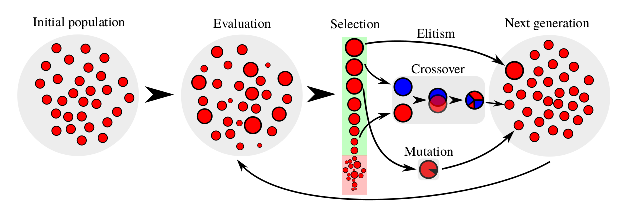
\includegraphics[width=0.8\textwidth]{../Figures/Misc/Evolution.eps}
\caption{Basic pipeline of an evolutionary method.}
\label{fig:evolutionPipeline}
\end{figure}


Figure~\ref{fig:evolutionPipeline} illustrates the general algorithmic pipeline of an evolutionary method, as described above. This starts with a random initialized population which is then evaluated (size refers to how ``good'' each individual is). All individuals are then sorted based on their goodness in respect the objective function. The selection process follows, where a set of the best individuals is selected to produce the next generation. Elitism, alongside crossover and mutation are used to this proportion of the population. The next generation will also be evaluated in respect to the same objective function and the iterative process will continue.

\section{Evolutionary Robotics}
\label{sec:evolutionary_robotics}

Evolutionary robotics~\citep{nolfi2001evolutionary} (ER) is a method that makes use of evolutionary computation algorithms to evolve the control and/or the morphology, without the direct design by engineers. Most research concentrates on developing robot controllers for simulated or real robots~\citep{harvey1997evolutionary,nolfi1994evolve}. One big advantage of this method is that it can evolve solutions for environments that designers and engineers do not have enough knowledge about (i.e., designing a robot controller for another planet, where surface type and gravity level might be crucial variables for the design of an exploring robot). In the same fashion as natural evolution, evolutionary techniques work with a population of random initialized controllers or designs. The candidate population individuals (robot controllers) used in ER applications may be drawn from some subset of the set of artificial neural networks (ANNs), whereas simpler versions of genetic algorithm applications use bit-streams that directly map the controller. The controllers in the best performing robots are then selected, altered and propagated through mutation, crossover, and other genetic operations, in a repeating process that mimics natural evolution. Evolutionary robotics is done with many different objectives, often at the same time. These include creating useful controllers for real-world robot tasks, reproducing biological phenomena, etc.. Creating controllers via artificial evolution requires a large number of evaluations of a large population. This usually takes a lot of computational time, which is one of the reasons why evolution of such controllers is usually evaluated within a simulation software. Initial random controllers may exhibit potentially harmful behavior, such as repeatedly crashing the robot into a wall, which may damage a physical robot.

Apart from evolutionary methods to develop robot controllers reinforcement learning~\citep{hayes1994robot,mahadevan1992automatic} can be used rewarding actions, resulting to state-action pairs that lead to high rewarding behaviors. As a result, a robot controller can be indirectly built. Applying evolved robot controllers to real robots in a physical environment is an extremely difficult task, since simulators in front of the limitations of computing efficiency sacrifice the accuracy~\citep{jakobi1995noise}. As mentioned earlier, evolutionary methods can be used to design the physical structure (morphology) of a robot~\citep{hiller2010evolving}, in addition to or in place of the controller. This thesis is exploring this aspect of evolution, the simultaneous evolution of the morphology and the locomotion of virtual soft robots. 

Developmental robotics~\citep{lungarella2003developmental,asada2001cognitive,weng2004developmental,asada2009cognitive} is a field related to evolutionary robotics,  while instead of evolving through generations towards fitter controllers, it is trying to mimic life-like learning starting from a ``blank'' state in which the robot's ``brain'' is initialized and every variable of the environment is unknown.

\begin{figure}[t!]
\centering
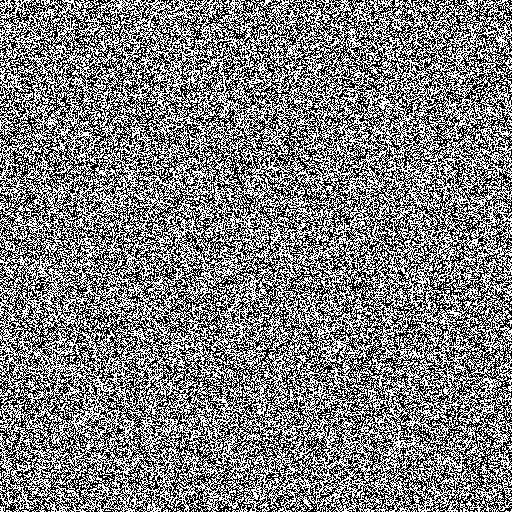
\includegraphics[width=0.3\textwidth]{../Figures/Misc/direct.jpg}\  \   \   
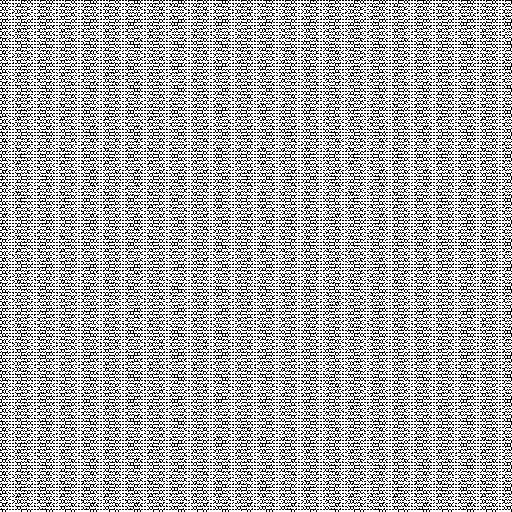
\includegraphics[width=0.3\textwidth]{../Figures/Misc/indirect.jpg}
\caption{Comparison of direct encoding versus generative for the binary image example.}
\label{fig:directVsIndirectEncoding}
\end{figure}


\section{Direct-Indirect Encoding of the Genotype}
\label{DirectIndirect}

A simple direct encoding was described in the previous section, when a single dimension stream of bits or numbers described the chromosome. When the dimensions of the task define the length of the genome, we refer to \emph{direct} encoding, which means that the genotype-phenotype mapping is a straightforward function. An example of this encoding could be the design of a two dimensional binary image. In direct encoding the genotype of this picture can be represented by a stream of bits which has the same length as the number of pixels of the image. In other cases, where there is no direct mapping between the genotype and the phenotype, indirect encoding is present, where a set of rules or a function maps the genotype to the phenotype space. In cases the phenotype space can be represented by a Cartesian n-dimensional space, an indirect encoded chromosome can be a function that is queried for each coordinate in a specific resolution and represents the phenotype. For the same binary image example, indirect encoding would be a function that gives pixel values $0$ or $1$ for every pixel's coordinate. 



Figure~\ref{fig:directVsIndirectEncoding} illustrates the difference between direct and indirect encoding. An example binary image is shown for both encoding schemes, in the first case (direct encoding) the genotype is a binary stream which length is equal to the number of pixels producing the value of each pixel directly. The latter encoding uses a genome of length 3, as many as the coefficients of the linear combination in the following function: 
\[f(x,y) = c_1 sin(x) + c_2 cos(x) + c_3 tan(y)
\]
the result is taken after applying the same function for each pixel coordinate. Even in cases where a simple function is used, the  phenotype holds some of its functions properties such as symmetry and repetition, resulting in a pattern that direct encoding cannot produce.

A method that can represent more complex functions and is widely used to indirectly map the genotype to the phenotype space is the \emph{artificial neural networks}. Artificial neural networks (ANNs) are computational models which are inspired by living-organisms central neural system (Brain). These models are used to approximate functions that are generally unknown, using a set of nodes and connections between pairs of nodes. Each connection within the network holds a weight which used as a multiplicative factor of each signal passing through the connection. Nodes are then responsible of propagating the summation of the signal received from the connections by a Sigmoid function. This interconnected set of nodes can propagate the inputs fed into the network to one or more output nodes, approximating in this way a complex non-linear function.


\begin{figure}[t!]
\centering
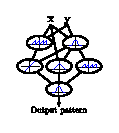
\includegraphics[width=0.25\textwidth]{../Figures/Misc/cppnNetwork.eps}
\caption{Compositional pattern-producing networks have identical network structure with artificial neural networks while they make use of a canonical set of activation functions.}
\label{fig:cppnNetwork}
\end{figure}



\subsection{Compositional Pattern-Producing Networks}
\label{CPPN}

Encoding plays an important role and it is critical to the performance of evolutionary algorithms especially when large problem spaces are present. Research has shown that the genotype-phenotype mapping can affect performance~\citep{komosinski2001comparison} in three dimensional agents, where more complex encoding schemes outperform direct encoding. In addition, geometrical implications of the problem also have some potentially important roles in the encoding. The role of symmetry to the encoding is crucial especially in applications like board games, robot controllers, biped walking, etc.. In these cases, geometric regularities of the encoding can be essential to the performance of the evolutionary method.

\begin{figure}[t!]
\centering
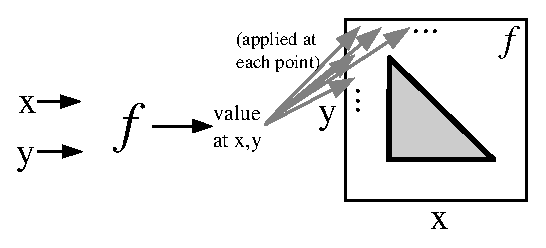
\includegraphics{../Figures/Misc/cppnResolution.eps}
\caption{CPPNs work as a function $f$ that is being queried for the whole n-dimensional Cartesian space in which space the phenotype is mapped, in this case the phenotype is the triangle in a two-dimensional space, figure taken by~\citep{stanley2007compositional}.}
\label{fig:cppnResolution}
\end{figure}

\emph{Compositional pattern-producing networks}~\citep{stanley2007compositional} or CPPNs are artificial neural networks with an extended set of activation functions (see Fig.~\ref{fig:cppnNetwork}). Results by this encoding show that regular patterns can be produced in this generative mapping from the genotype to the phenotype space. Like in the previous two dimensional image representation of a phenotype, CPPNs generate phenotypes that can be interpreted as distributions of points in a multidimensional Cartesian space. The genotype (CPPN) can then be queried for each coordinate of the space and gives the phenotype representation of the genotype in multiple resolutions. In the same fashion, images can be constructed using CPPNs, where pixel coordinates are queried to the network and the grayscale or RGB values can be taken by the outputs of these networks. 


Figure~\ref{fig:cppnResolution} illustrates how the mapping between the genotype and phenotype is done using generative encoding (CPPNs). A major asset of CPPNs is that they can generalize in all resolutions. Considering the previous figure (see Fig.~\ref{fig:cppnResolution}), the CPPN is queried for all $x,y$ coordinates of the phenotype two dimensional Cartesian space. The step of $x,y$ sampling can be determined by the problem, since the inputs of the CPPN are the normalized coordinates $x,y \in [-1,1]$. Hence, genotypes using this kind of generative encoding can be mapped in every resolution, making this process straighforward to generalize. As the space of the phenotype becomes larger, a generative encoded solution (CPPN) is not affected by the increasing dimensions of the problem, a constraint that heavily affects direct encoding.

\begin{figure}[t!]
\centering

\includegraphics[width=0.25\textwidth]{../Figures/Misc/picBreed3.jpg}\quad   
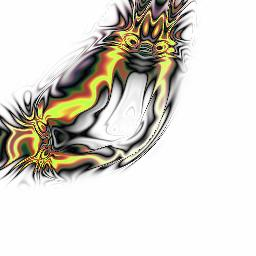
\includegraphics[width=0.25\textwidth]{../Figures/Misc/picBreed2.jpg}\quad
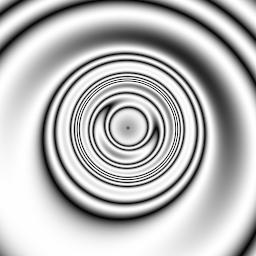
\includegraphics[width=0.25\textwidth]{../Figures/Misc/picBreed1.jpg}\\
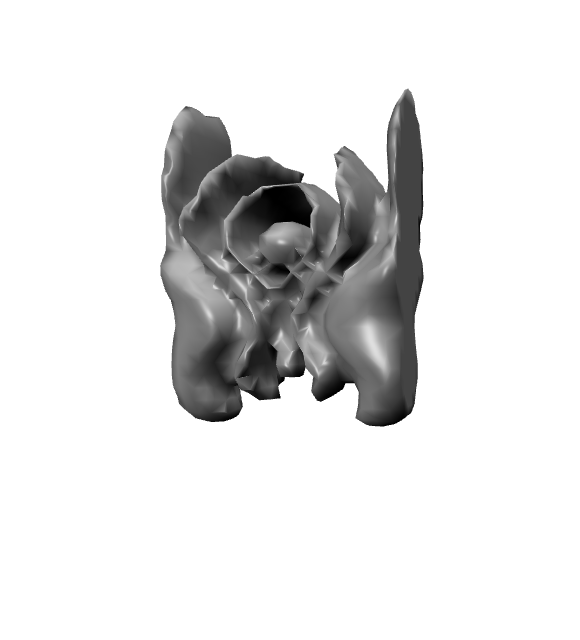
\includegraphics[width=0.25\textwidth]{../Figures/Misc/endless2.png}\quad 
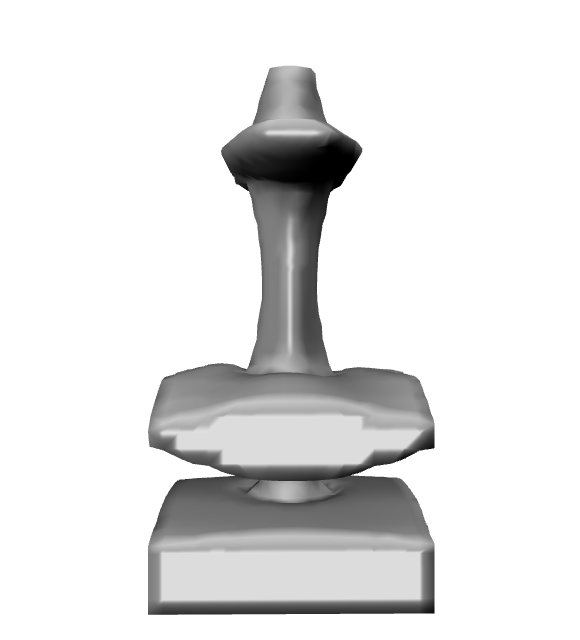
\includegraphics[width=0.25\textwidth]{../Figures/Misc/endless1.png}\quad
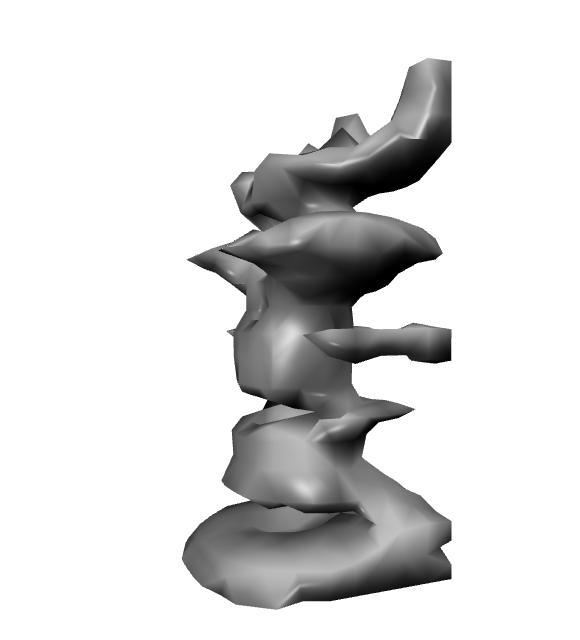
\includegraphics[width=0.25\textwidth]{../Figures/Misc/endless3.png}
\caption{Compositional pattern-producing networks can encode truly complex images\protect\footnotemark[1] (top) and 3D-structures\protect\footnotemark[2] (bottom).}
\label{fig:cppnImages}
\end{figure}

\footnotetext[1]{picbreederSite: \url{http://www.picbreeder.org}}
\footnotetext[2]{EndlessForms: \url{http://www.endlessforms.com}}

Compositional pattern-producing networks have been used in many applications where symmetry and repetition can produce two or three dimensional artistic structures\footnotemark[2], and drawings\footnotemark[1]~\citep{secretan2008picbreeder}. As these applications require more symmetrical properties than others, not only Cartesian space coordinates are fed into the inputs of these networks, but more inputs biasing the network should be present~\citep{secretan2008picbreeder}. Some example inputs that can be fed into the network as additional inputs are the distance from the center of the space or the distance from the center to one axis. Figure~\ref{fig:cppnImages} illustrates images encoded by CPPNs. Comparing the results with Figure~\ref{fig:directVsIndirectEncoding}, it is understandable why this kind of encoding can capture solutions in problem domains where symmetry is important.




\section{Neuroevolution}

\emph{Neuroevolution}~\citep{yao1997new} is an optimization technique using evolutionary methods as described in Section~\ref{sec:evolutionary_robotics}, where artificial neural networks take the place of simpler encoding methods. ANNs can compute arbitrarily complex functions, learn and perform under the presence of noisy inputs and generalize to unseen sensory information. Neuroevolution requires only a measure of a network's performance at a task, which can be used as the reward for good solutions (ANNs) to survive. More complicated forms of chromosome representations can develop more complex robot controllers. After each run, the sensory input of the task domain is given at the artificial neural network's input neurons and the solution is given by the output of the networks where the fitness of the specific brain can be evaluated. A major issue is the selection of the network's \emph{topology}. Topology is the arrangement of the network's elements such as links and nodes, which represents the structure and how the information flows within the network. In early neuroevolution methods the topology of the networks used was fixed, meaning that the only elements of the networks evolving were the weights of the connections between the nodes. In modern neuroevolution methods, the topology of the networks is also subject to the evolution.

\begin{figure}[t!]
\centering
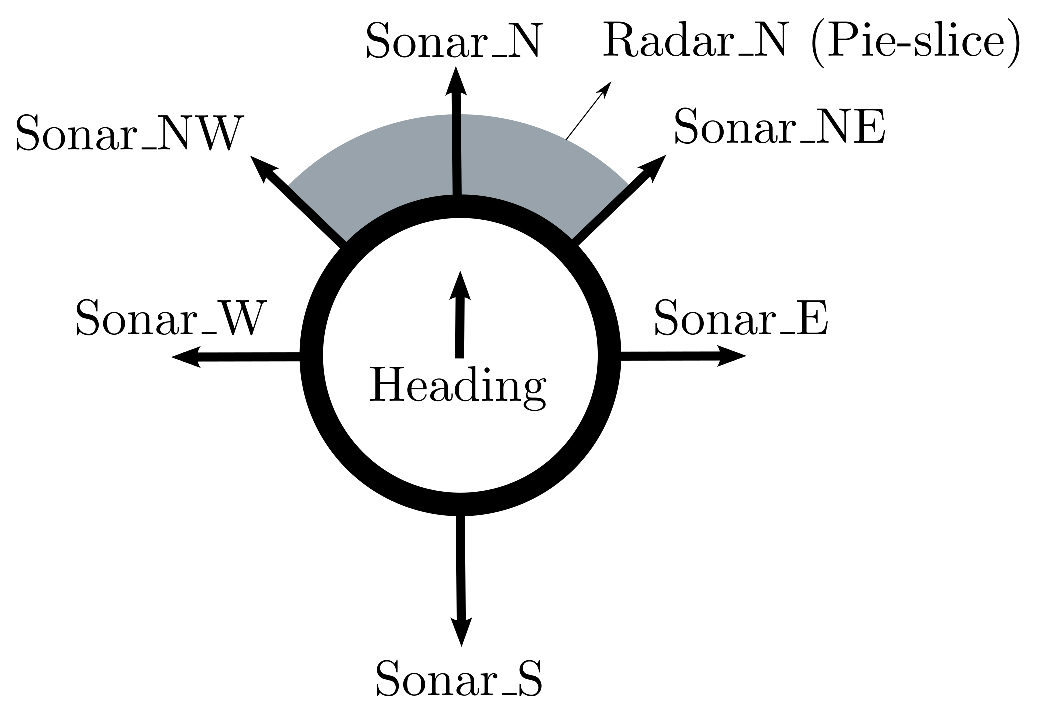
\includegraphics[width=0.35\textwidth]{../Figures/Misc/RobotMaze.eps}\  \    \  \    
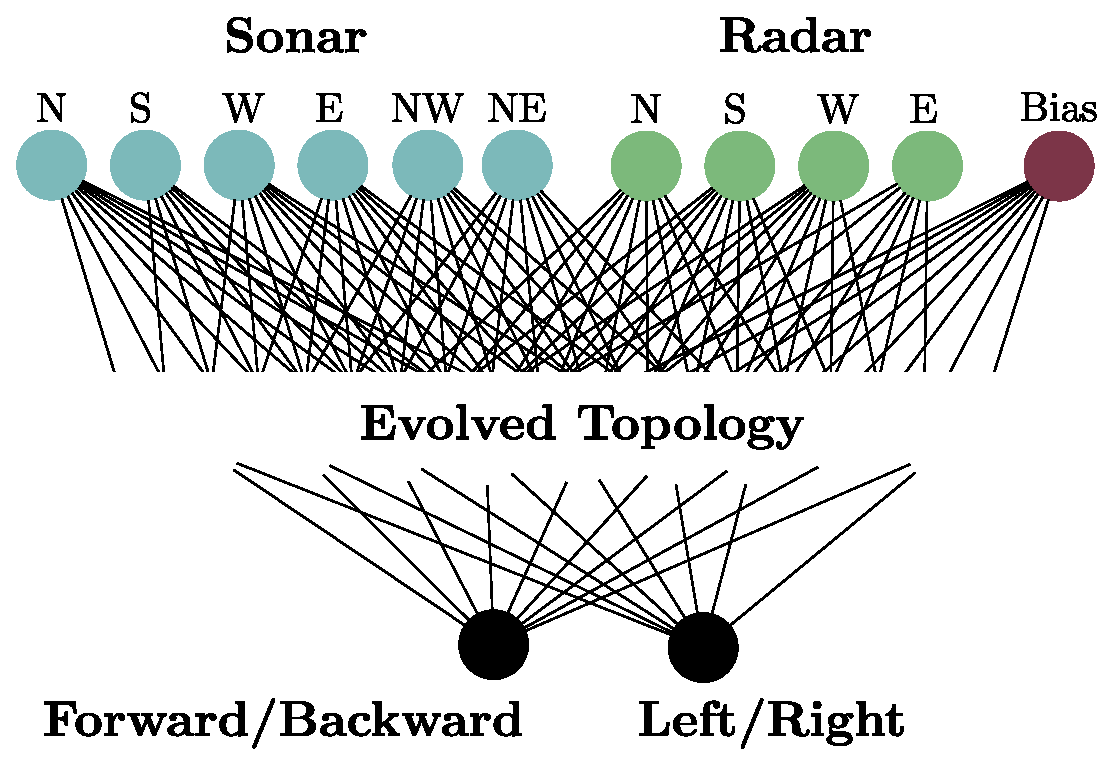
\includegraphics[width=0.49\textwidth]{../Figures/Misc/RobotMazeNetwork.eps}
\caption{Robot controllers can be evolved through neuroevolution algorithms where robot sensors are the inputs of neural networks while the outputs directly control the robot.}
\label{fig:robotExample}
\end{figure}


\subsection{Neuroevolution of Augmented Topologies}
\label{NEAT}

Neuroevolution of augmented topologies (NEAT) as it was first introduced by~\citep{stanley2002evolving} is also a neuroevolution method used to evolve artificial neural networks. A major advantage of this method is that alongside the weights it also evolves the topologies of the networks within the population.

Originally, neuroevolution methods were developed to capture difficult sequential decision making, as well as to control problems. The sensory information is the input of these neural networks and decisions are the outputs. NEAT is yet another method for evolving ANNs where a few extra features are added, enables finding solutions in more demanding problems. NEAT starts the evolution process with a population of networks with simple topologies. Through the generations instead of just fixing the weights of the networks' connections, topologies are becoming more complex allowing nodes and links to be added. Meaning that during the evolution, more complicated networks will be produced, this \emph{complexifying} technique leads to capturing more demanding solutions as it offers enough freedom to the evolution.

Figure~\ref{fig:robotExample} illustrates how sensory information can be given as input to a neural network. The neural network, given the sensory information provided, controls the robot which tries to drive itself close to a target position in a maze. The outputs of the network completely control the motion of the robot. All the sensory information (six sonar sensors which output the distance from the closest obstacle in six directions and 4 pie-slice radar sensors which are only activated when the target position is located within the range of each one covers) is available to the controller.

Several aspects of this method worth mentioning where \emph{speciation} is one of the most important. Speciation is the procedure that protects new \emph{species} until they have enough time to evolve before comparing them with the rest of the population. For two individual genotypes (ANNs) to belong to the same species their network topology must be similar, meaning that a threshold is set and a function determines the numeric value of two network topologies' similarity. Two different genotypes (ANNs) can share shame genes (topologies within the network) and their compatibility (genotype similarity) is given by:
\begin{equation}
\label{CompatibilityEquation}
\delta = c_1 \cfrac{E}{N} + c_2 \cfrac{D}{N} + c_3 \bar{W}
\end{equation}
where $E$ is the number of \emph{Excess} genes (genes that do not match and they do not occur in parents' genotype), $D$ is the number of \emph{Disjoint} genes (genes that do not match but they occur in parents' genotype), $\bar{W}$ is the average weight difference between \emph{Matching} genes (Identical) and $N$ is the number of genes in the larger genotype used for normalization.
The age of each species protects them for competing in equal terms with more optimized species, giving them in this way time to evolve further towards the objective function.



\section{CPPN-NEAT}

Compositional pattern-producing networks as described earlier in this chapter (see Sec. \ref{CPPN}) are similar computational methods to ANNs in regards to their structure, so one can make use of the \emph{complexifying} property to capture in this way more complex solutions (behaviors). NEAT method can evolve CPPNs in the place of ANNs, since it only needs few modifications. 

The resulted method that evolves this generative type of genomes (CPPNs) is called CPPN-NEAT~\citep{stanley2007compositional} and its only difference in respect to the original NEAT algorithm is the way new nodes are added to the network. The original NEAT algorithm evolves ANNs which are using sigmoid functions at every node, so every new node will carry this function.
In the contrary, CPPNs use a variety of functions from a canonical set. CPPN-NEAT assigns a random function from this set to every newly added node. 

Experiments~\citep{stanley2007compositional} have shown that this method can indeed evolve CPPNs capturing in this way solutions in problems with geometrical properties (i.e board games, biped walking, etc.). NEAT is holding the properties of natural evolution as every neuroevolution method. Furthermore, NEAT coupled CPPN encoding can be used to determine the connectivity (topology) of artificial neural networks in  a method called HyperNEAT~\citep{stanley2009hypercube}.




\section{Novelty Search}
\label{NoveltySearch}

Traditional search within the framework of evolutionary algorithms needs an objective function, a function that guides the search towards ``good'' areas of the solution space following the gradient of the fitness. Defining the fitness function is a straightforward problem most of the time. In a problem where a robot tries to get to a target from its initial position in a room with no obstacles in between a fitness function could be defined as the Euclidean distance between the final position of the robot and the target point, the closer it gets to the target the more points (higher fitness) the specific controller is rewarded.

\subsubsection*{When the objective function misleads the search}

\begin{figure}[t!]
\centering
\begin{subfigure}[b]{0.3\textwidth}
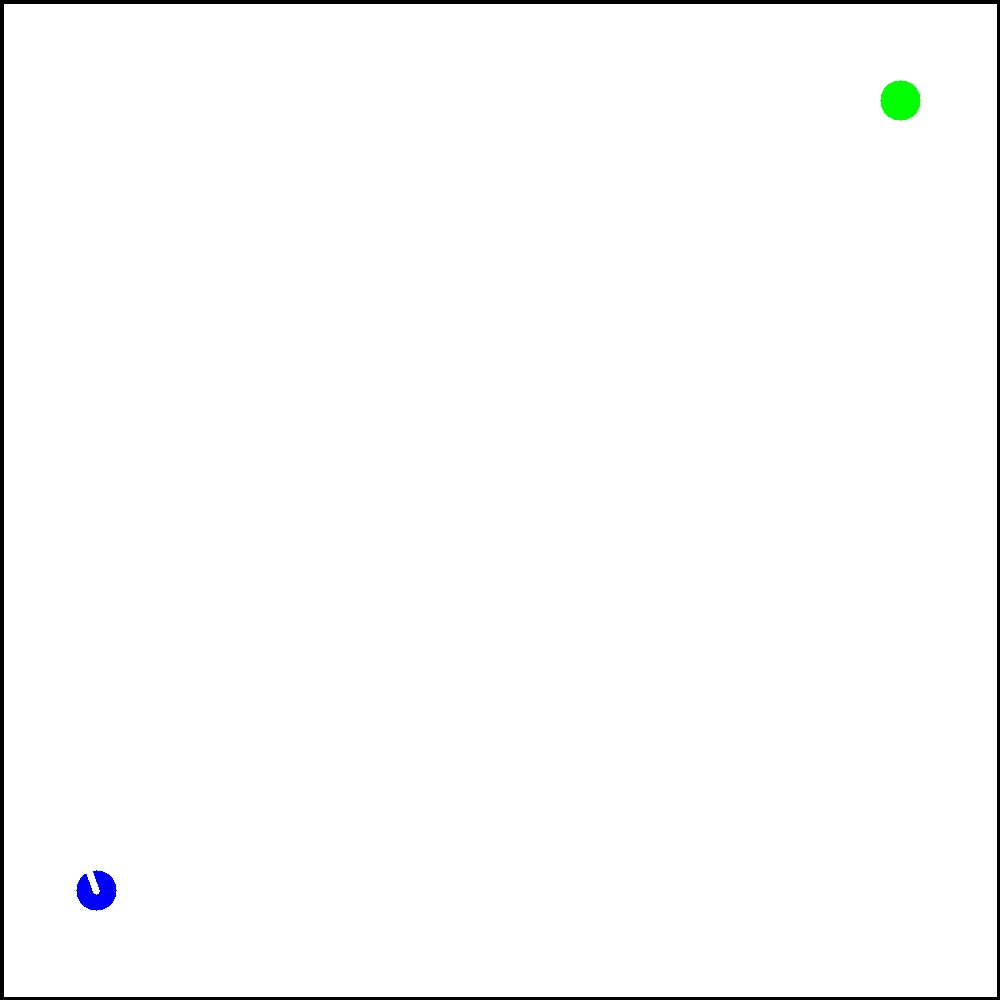
\includegraphics[width=1.0\textwidth]{../Figures/Misc/MazeEasy.jpg}
\caption{Easy}
\label{fig:mazeEasy}
\end{subfigure}\hspace{2cm} 
\begin{subfigure}[b]{0.3\textwidth} 
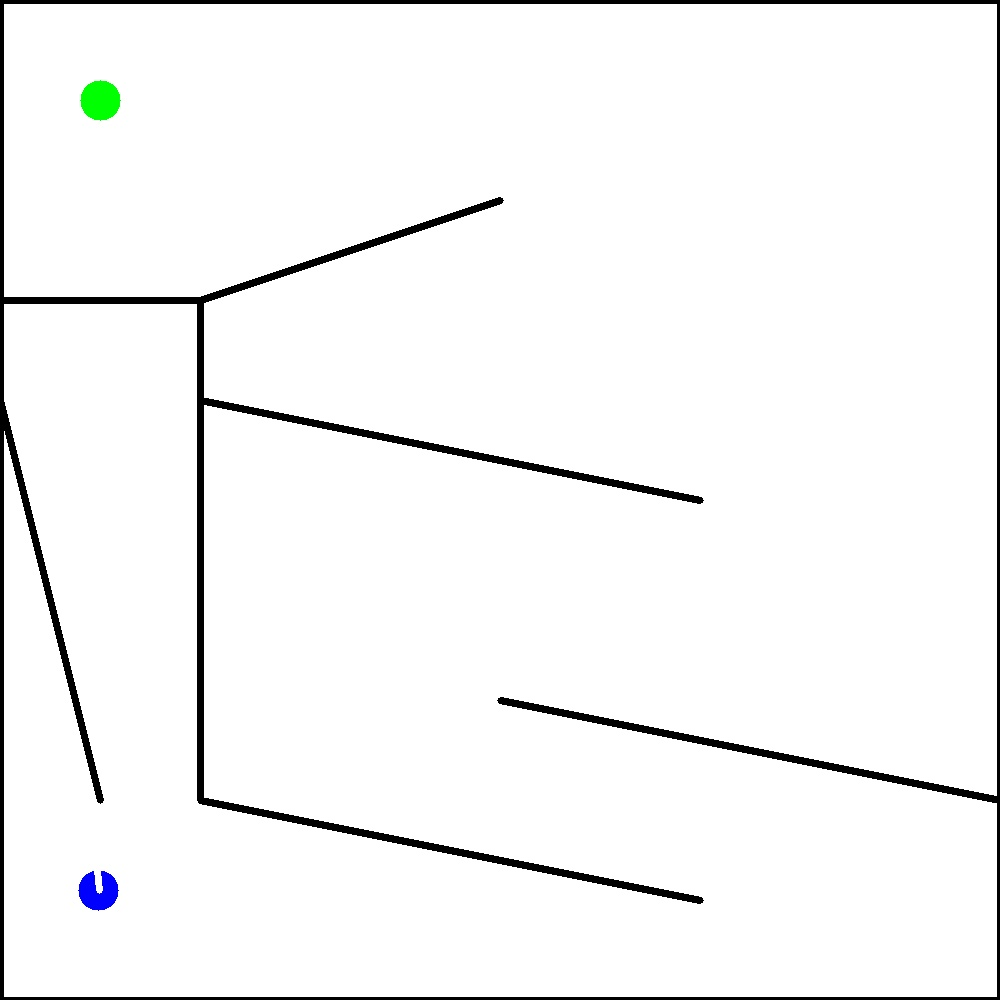
\includegraphics[width=1.0\textwidth]{../Figures/Misc/MazeHard.jpg}
\caption{Hard}
\label{fig:mazeHard}
\end{subfigure}
\caption{An objective function can be devious. Maze examples from~\citep{lehman2011abandoning}.}
\label{fig:maze}
\end{figure}

An objective function as the one described above is greedy, driving the search directly towards highly rewarding areas of the solution space. In cases that local optima can be found in the landscape of the objective function this greedy fitness measure can drive and trap the evolution in these localities of the problem.

Considering the robot-maze example presented in~\citep{lehman2011abandoning,lehman2010revising}, a robot (\textcolor{Blue}{blue} dot) is placed in a maze (see Fig.~\ref{fig:maze}), the robot (see Fig.~\ref{fig:robotExample}) has multiple sensory information which are fed as inputs to its controller (``brain''). The controller is driving the robot through the maze having only sonar and radar sensory information, while its ultimate goal is to drive the robot to the target position (\textcolor{Green}{green} dot) in a fixed time span. Naturally, to select a fitness function that can give enough information about how good a controller is the Euclidean distance  from the final position of the robot to the target position is measured in the end of the simulation time. For the first maze (see Fig.~\ref{fig:mazeEasy}) when no obstacles are between the robot and its target the objective function is reliable, since the Euclidean distance to the target indeed informs the robot how close it is located. In the second maze (see Fig.~\ref{fig:mazeHard}) using the same fitness function search can be mislead. In this example maze achieving high fitness does not mean that the robot is actually close to the target. Driving north in this maze following the increasing fitness leads to a wall that cannot be passed by the robot. Therefore, exploration is needed in low fitness areas which will allow the robot to reach the target point with the maximum fitness. The deceptive nature of the fitness function in this problem can be found in a lot of optimization problems, while the walls in this maze clearly denote problems where this fitness landscape can be found. 

\begin{figure}[t!]
\centering
\begin{subfigure}[b]{0.3\textwidth}
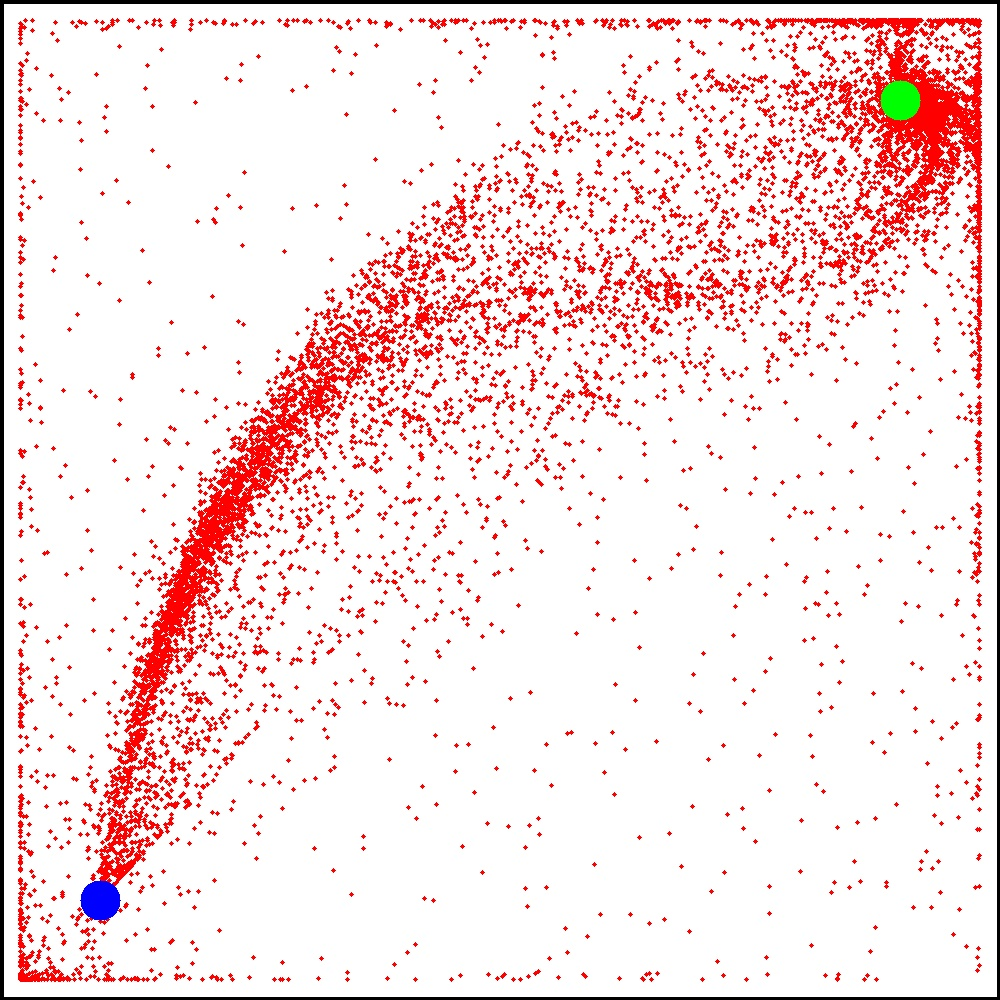
\includegraphics[width=1.0\textwidth]{../Figures/Misc/MazeEasyFitness.jpg}
\caption{Visited space after $200$ generations.}
\label{fig:mazeFitnessEasy}
\end{subfigure}\hspace{2cm}
\begin{subfigure}[b]{0.3\textwidth}
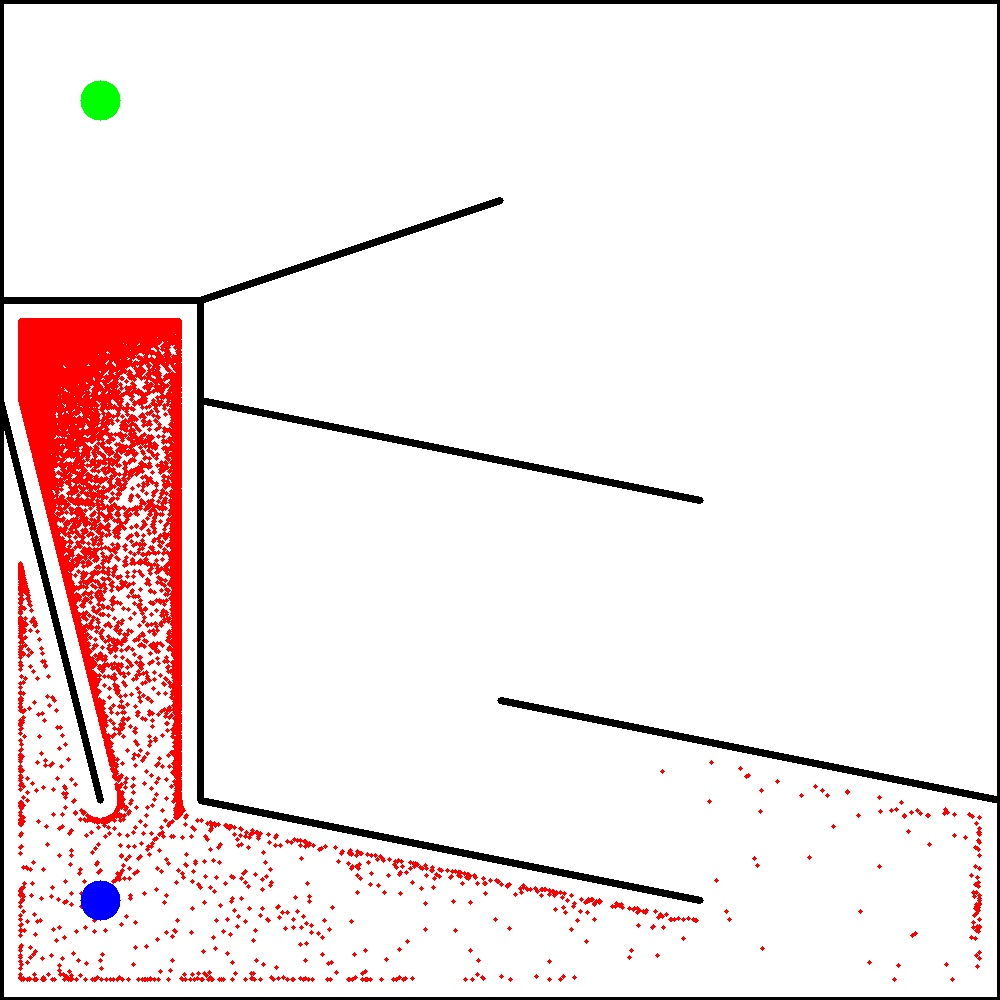
\includegraphics[width=1.0\textwidth]{../Figures/Misc/MazeHardFitness.jpg}
\caption{Visited space after $1000$ generations.}
\label{fig:mazeFitnessHard}
\end{subfigure}
\caption{Fitness search has no problems to find the solution in the easy map, while it can not find the optimal solution in the hard setting after $250.000$ evaluations.}
\label{fig:mazeFitness}
\end{figure}


To visualize how fitness based search can fail in such a setting Figure~\ref{fig:mazeFitness} presents the results of the above experiment explained using the robot sensory information presented in Figure~\ref{fig:robotExample}. NEAT algorithm is used to evolve the neural controller presented in the same figure. The settings used for this experiment were the same as in~\citep{lehman2011abandoning} where a population of $250$ individual controllers per generation was used. As it was expected, fitness based search was successful in the easy setting (see Fig.~\ref{fig:mazeFitnessEasy}). However, it failed to find the optimal solution in the hard map (see Fig.~\ref{fig:mazeFitnessHard}) focusing on creating controllers that lead the robots drive north until the wall was reached, failing to explore the map extensively.

\subsubsection*{Natural evolution is not an evolution towards fitness}

Using an objective function in evolutionary computation and typically reward individuals which are closer to an objective is far away from natural selection in the evolution process, where exploration is allowed as long as the criteria for survival hold~\citep{lehman2010revising}. Driving search towards promising parts of the fitness space where local optima may be present ensures that other areas of the search will not be explored, leading search to stay and explore the nearby area while more promising regions are far away in the solution space. Solutions located in these regions are called \emph{stepping stones}~\citep{lehman2008exploiting,lehman2011abandoning,lehman2010revising,risi2009novelty}. Stepping stones are points in the solution space that may not be good as far as their objective values are concerned, but can eventually lead to better or the global optima of a specific optimization problem.


\subsubsection*{Search for novelty}

Novelty search~\citep{lehman2008exploiting,lehman2011abandoning,lehman2010revising, risi2009novelty} unlike traditional fitness based search is an alternative way of optimization towards an objective function without having knowledge of this objective. In simple words it is looking for a solution to a problem without knowing how close it is to solve it; fact that turns out to have a major impact to the increased performance of this method in several problem domains. 

What novelty search seeks for is how interesting a new solution is in respect to all previously found ones. To define ``interesting'' we need to move our point of interest into behavior space which is a function of each phenotype, similar to the fitness function. Nevertheless, it fully or partially describes the behavior without directly implying the fitness function. As an example someone can think of a behavior could be defined as the final position of the navigation robot or the trajectory of it in the previous robot-maze example. Rewarding behaviors of the phenotype that are different from the previously found ones drives the evolution to visit new points in the behavior search space.

One significant point here is that the behavior space in some domains can be limitless. However, a valid behavioral metric can be found excluding behaviors that are meaningless or do not comply with the natural limits of the problem. On the other hand, the search space in the genotype level can also be infinite especially in neuroevolution methods like NEAT where ANNs can grow during the evolution. A bounded space of understandable-valid behaviors is then the key idea of novelty search where increasingly complex behaviors present to the evolution as the complexity of the genotype grows along.

Multi-objective optimization can also make use of a novelty metric alongside fitness, trying to optimize both at the same time~\citep{mouret2011novelty}. Another method that exploits the diversity of the produced genomes in order to map the phenotype to the fitness is also proposed by the literature~\citep{mouret2012algorithm}.

\subsubsection*{Is novelty search similar to random?}

Initial thoughts are converging that novelty search is similarly behaving to random search, constantly looking for something new in the vast space of behaviors. It seems similar to evolving random robot controllers without considering the behavior aspect of their phenotypes hoping that enough exploration will be done in both genotype and phenotype spaces. A random approach having no information about the observed behaviors the evolved phenotypes produce is not able to drive the evolution since different and more complex genotypes can easily produce similar behaviors. The novelty in the behavior level assures that the search will explore deeply the behavior space with the hope that a \emph{fit} behavior will be found. Aside from that, novelty search does not perform backtracking which ensures that it will constantly drift away from already generated behaviors (i.e similar behaviors to already generated ones result to low novelty value). At the same time there is no such guarantee in random search. Therefore, it is certain and proven later in this thesis that no exploration in the behavior space will be performed by random search.



\subsubsection*{How can novelty be measured?}

As fitness is a function to measure the ``goodness'' of an individual, novelty measures how different an individual is from all previously found individuals. To define different a novelty metric measures the difference in the behavior space of the phenotype. Given the phenotype's behavior $x$ a novelty measurement could be a function of $x$, $f(x)$ which computes how different (novel) is the specific behavior in respect to a set of other behaviors $S$ in behavior space.  As defined in~\citep{lehman2008exploiting,lehman2011abandoning} \emph{sparseness} can give a good measurement of how sparse is the area of a newly observed behavior. Given the behavior we can compute the sparseness by:
\begin{equation}
\label{sparsenessEquation}
f(x) = \cfrac{1}{k} \sum_{i=1}^{k} dist(x, S_i)
\end{equation}
where $S$ is a sorted set of the closest behaviors. Sparsity measures the average distance from the $k$-closest behaviors.


\subsubsection*{Algorithm}

\begin{figure}[t!]
\centering
\begin{subfigure}[b]{0.3\textwidth}
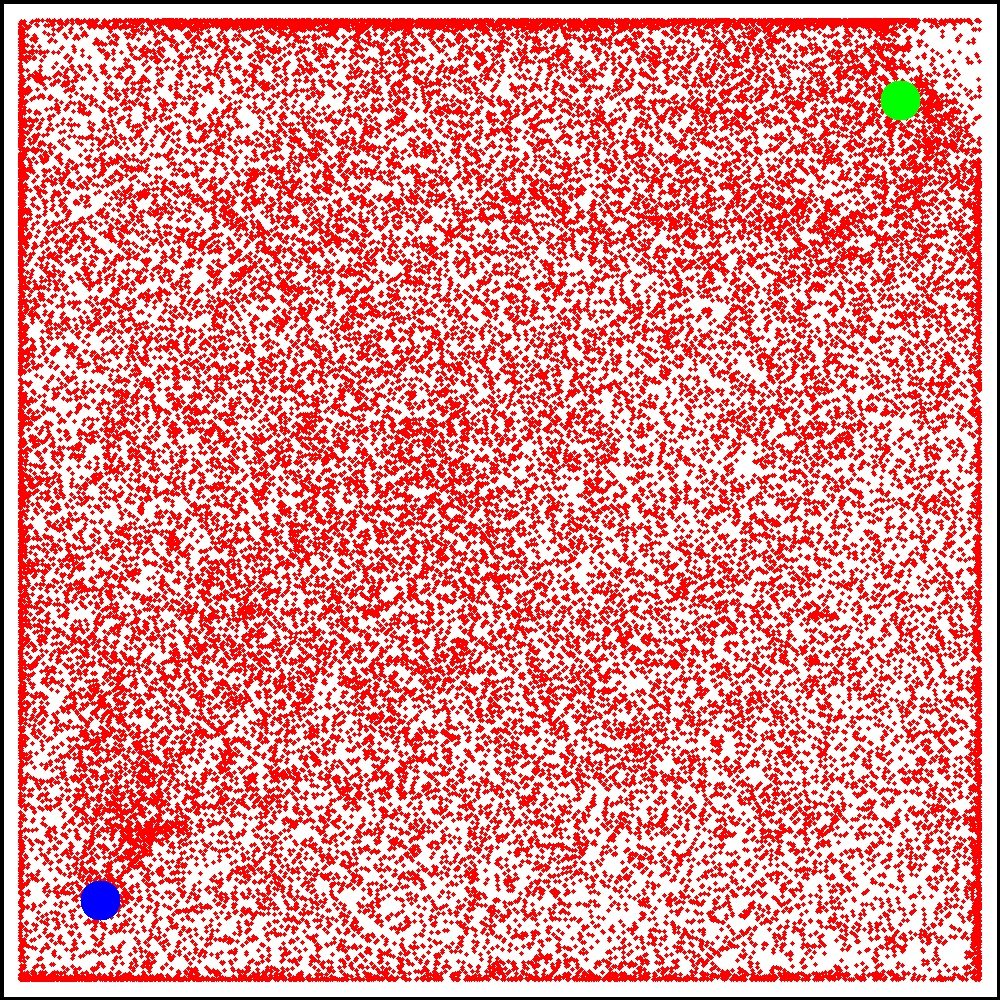
\includegraphics[width=1.0\textwidth]{../Figures/Misc/MazeEasyNovelty.jpg}
\caption{Visited positions in the map after $200$ generations.}
\label{fig:mazeNoveltyEasy}
\end{subfigure}\hspace{0.3cm}
\begin{subfigure}[b]{0.3\textwidth}
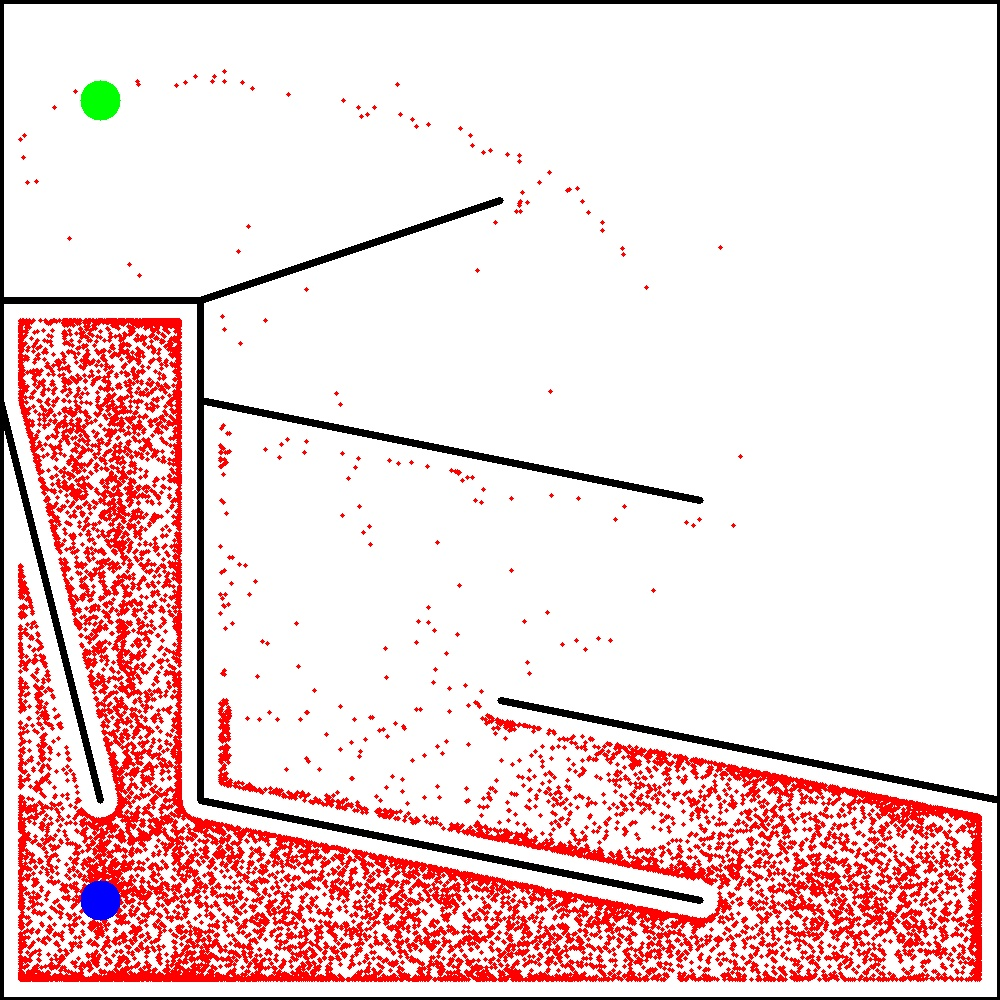
\includegraphics[width=1.0\textwidth]{../Figures/Misc/MazeHardNoveltySolution.jpg}
\caption{Solution found after only $80$ generations.}
\label{fig:mazeNoveltyHardSolution}
\end{subfigure}\hspace{0.3cm}
\begin{subfigure}[b]{0.3\textwidth}
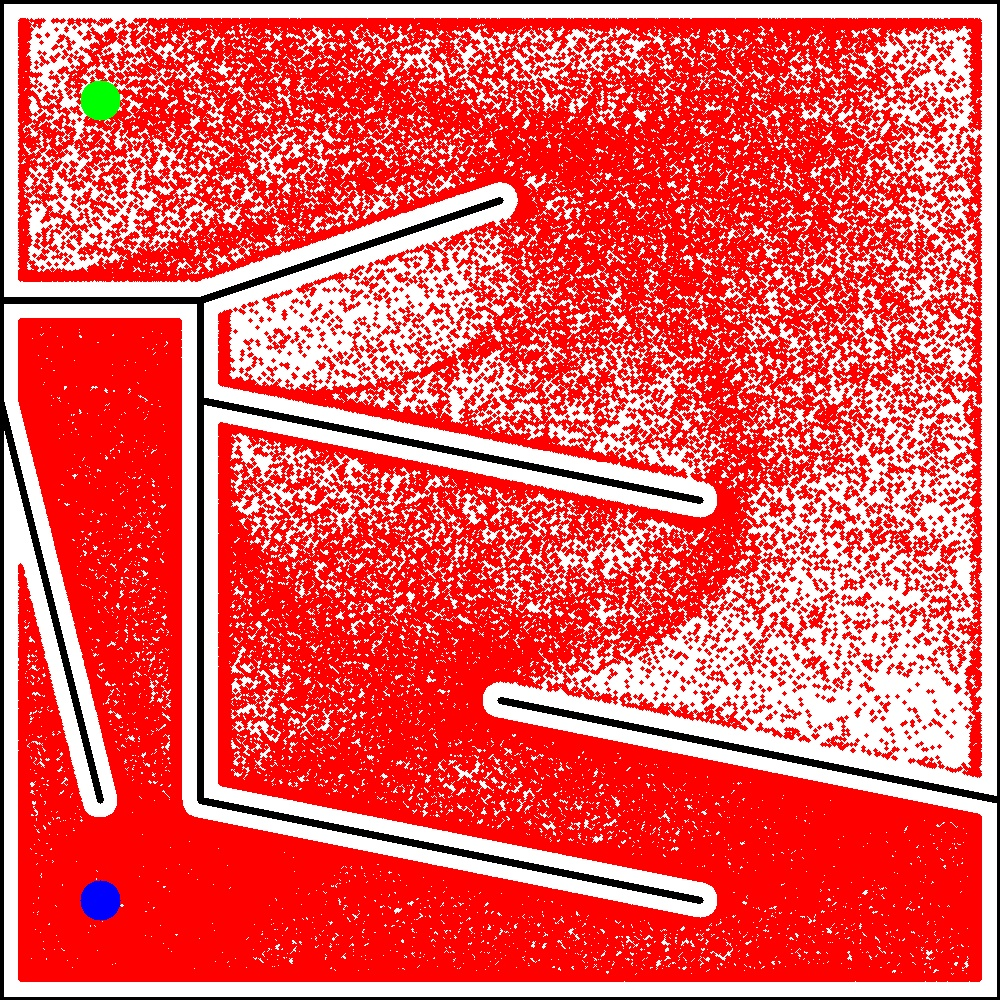
\includegraphics[width=1.0\textwidth]{../Figures/Misc/MazeHardNovelty.jpg}
\caption{ Visited positions in the map after $1000$ generations.}
\label{fig:mazeNoveltyHard}
\end{subfigure}
\caption{Novelty search applied in the robot-maze optimization problem. Novelty search deeply investigates the behavior space finding the solution even in the hard map setting.}
\label{fig:mazeNovelty}
\end{figure}


Replacing fitness with a novelty value is not the only modification any evolutionary algorithm needs in order novelty search to be implemented. To push search to visit new areas in the behavior space rewarding novel behaviors coming up during the evolution is needed. For this reason, storing novel reference points in space (behaviors) during the evolution is inevitable. The sparseness of a new behavior is computed by Equation~\ref{sparsenessEquation} resulting in a numerical value that implies how novel is the observed behavior of an individual phenotype. If the new behavior has a novelty value more than this threshold it is stored in the set of novel individuals. Apart from comparing any new behavior with all the novel behaviors, the newly produced one can also be confronted with the entire set of behaviors produced by the population in the same generation of the evolution. 

Having discussed the basic idea behind novelty search and how it can be implemented, it is time to apply it in a known problem where fitness based search failed. Considering the robot (see Fig.~\ref{fig:robotExample}) - maze (see Fig.~\ref{fig:maze}) example presented in this section, novelty search is now taking the place of evolution towards the objective function used before which was the distance to the goal. For the novelty metric to be evaluated, a behavior metric has to be defined, which in this case can be the final position of the robot by the time the simulation is finished. The sparsity measure then computes the reward of the robot based on how sparse the observed behavior of the robot in regards to all novel behaviors found before in the evolution is, based on the sparsity equation (see Eq.~\ref{sparsenessEquation}) using $k = 10$. Figure~\ref{fig:mazeNovelty} presents the results achieved by novelty search in this setting by showing all the visited areas that robots were driven to by their evolved controllers. In the easy setting map (see Fig.~\ref{fig:mazeNoveltyEasy}), novelty search achieved to fully explore every possible position in the map. In the hard map (see Fig.~\ref{fig:mazeNoveltyHardSolution}, \ref{fig:mazeNoveltyHard}), where fitness based search failed to find any solutions close to the target position, novelty search succeeded to do so after only $80$ generations.



\section{Soft Robotics}
Soft robotics is a highly promising field of research dedicated to the science and engineering of soft materials in mobile machines. As the name suggests soft robots~\citep{trivedi2008soft, pfeifer2012challenges} are made entirely of soft materials mimicking animals or animal-parts that consist only of soft tissue (elephant trunk, tongue, worm, octopus, etc.). Having no rigid parts in their design the degrees of freedom are infinite and the possible ways of motion can become extremely complex. In traditional robotics, joints and rigid parts predefine the space of possible movement and sometimes restrict the robot's locomotion strategy or \emph{gait} to a specific set. In soft robotics, the absence of rigid parts can on the one hand make the design of the locomotion strategy exceptionally tortuous, on the other hand the gait alternatives are limitless.

\begin{figure}[t!]
\centering
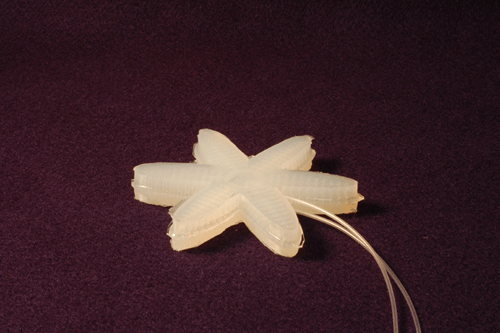
\includegraphics[width=0.3\textwidth,height=0.13\textheight]{../Figures/Misc/soft_robotics_figure.png}\		
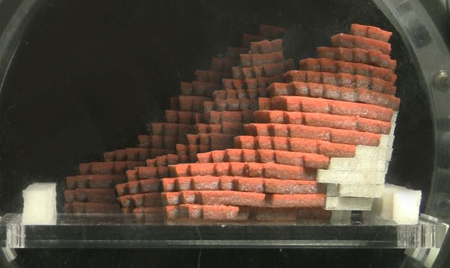
\includegraphics[width=0.3\textwidth,height=0.13\textheight]{../Figures/Misc/hillerPressureChamber.png}\	
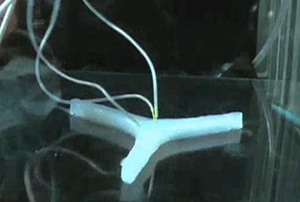
\includegraphics[width=0.3\textwidth,height=0.13\textheight]{../Figures/Misc/ExplodingRobot.jpg}\\
\caption{Soft robots can be actuated through air pressure tubes (left), pressure variations (middle), or internal explosions (right).}
\label{fig:softRobotsActuation}
\end{figure}

The design and development of soft robotics is not an easy task, while the actuation of such soft structures is the most challenging task. Actuating soft materials can be done in many ways including pneumatic systems~\citep{ilievski2011soft, shepherd2011multigait}, hydraulic, internal body explosions, passive actuation triggered by pressure or temperature variations and others~\citep{laschi2012soft, seok2010peristaltic}. Figure~\ref{fig:softRobotsActuation} illustrates three different ways that soft robot bodies can be actuated. Gripping mechanisms~\citep{hirose1978development} can softly and gently conform to objects of any shape and hold them with uniform pressure. This gripping function is realized by means of a mechanism consisting of links and series of pulleys which can be simply actuated by wires. Regardless traditional ways of actuating soft material robots, three dimensional printing is now giving the freedom for multi-material structures to be created, which also explodes the number of possibilities for the design of a soft structure such as a gripper soft robot. Topological optimization techniques can be applied~\citep{hiller2009multi} for producing functionalities in the design. Autonomously actuated soft robots~\citep{tolleyresilient} (see Fig.~\ref{fig:softbot}) can also be designed having multiple advantages over rigid body robots such as resistance under extreme temperatures and the capability of locomotion on terrains of variant types. 

Although soft robotics research field is in an early stage, it is growing fast. Some of the characteristics that make soft robots interesting to explore are the infinite number of degrees of freedom and the variety of materials (mostly elastic) that can be used, in the contrary to rigid robotics that are mostly made out of metals and plastic. Nevertheless, structure design and control of soft robotics remain challenging mostly because of their soft bodies can only be represented in continuous state spaces, where only analytic methods can be proven successful.

To sum up, locomotion capabilities of soft robots, as well as the possibilities of passive movement (i.e materials that actuate reacting to environmental changes) makes them an interesting topic for present and future research. Finally, considering also that soft materials are safer than conventional robot materials to humans, human-robot interaction can benefit from this field~\citep{sanan2011continuum}.


\begin{figure}[t!]
\centering
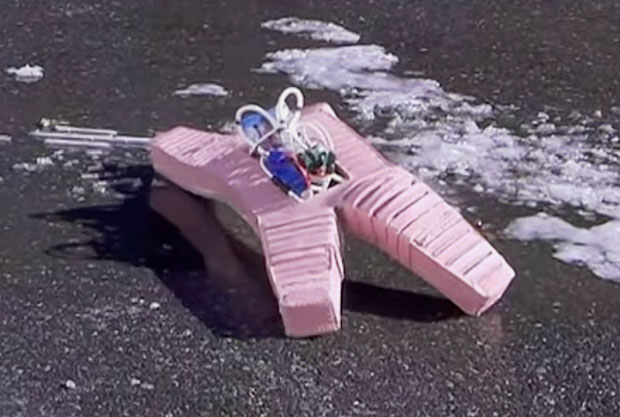
\includegraphics[width=0.6\textwidth]{../Figures/Misc/softbot.jpg}
\caption{Autonomously actuated soft robot~\citep{tolleyresilient}, it is able to withstand extreme temperatures and variant terrain types.}
\label{fig:softbot}
\end{figure}


\subsection{Soft Robotics in Simulation}

Most work to simulate interactions and deformations within and between soft material bodies are mostly focused on the graphical part of the problem~\citep{faloutsos1997dynamic} sacrificing the accuracy of the simulation~\citep{teschner2004versatile}. Three dimensional meshes~\citep{muller2002stable} can represent these bodies including the dynamics of their materials. 

A recent work though, \emph{VoxCad} simulator~\citep{hiller2012dynamic} is focusing mostly on the physics side of the soft material interactions not at the expense of a low frame rate. \emph{VoxCad} is a modeling and analyzing open-source software that can simulate soft material deformations and interactions. In Figure~\ref{fig:VoxCAD} the graphical user interphase of VoxCad software is presented during the simulation of the soft body robot in the simulator.

VoxCad cannot model and simulate three dimensional meshes, yet a lattice is used to represent the 3D workspace where voxels (three dimensional pixels) can be assigned different materials. Materials themselves are passive and cannot actuate without external trigger. In this simulator this external force that can actuate the materials is the temperature of the environment. The main variables of the environment is the base, the amplitude and the period of the temperature. Furthermore, gravity acceleration of the environment can vary. Materials have properties such as the elasticity of the material, density, Poisson's ratio, coefficient of thermal expansion (which determines how materials will be expanded in respect to the environment's temperature), temporal phase in respect to the temperature period, and the ground friction coefficients. Materials can also be mixed together to create a new type of material.

\begin{figure}[t!]
\centering
\includegraphics[width=1.0\textwidth]{../Figures/Misc/voxcad.png}
\caption{VoxCAD (Voxel CAD), a cross-platform open source voxel modeling and analyzing software.}
\label{fig:VoxCAD}
\end{figure}

Throughout this thesis, the terms \textit{structure} or \textit{soft robot} will refer to a set of connected voxels (not unconnected parts) within the lattice space. The voxel dimensions are constant through the experiments of this thesis, while the lattice space is variant. Since the voxel dimensions are the same for all settings, the term \textit{resolution} will be referring to the number of voxels in each dimension. Note that different resolutions also refer to different dimensions for the lattice as the voxel size is fixed.  For experimental settings used during the simulations see appendices~\ref{SimulationSettings}, \ref{ExperimentalSettings}. 




\begin{comment}
\section*{\todo{Additional Material that can be added later}}
\citep{stanley2003taxonomy}
\citep{nelson2009fitness}
\citep{meyer1998evolutionary}
How the Body Shapes the Way We Think A New View of Intelligence~\citep{pfeifer2007body}
\citep{albu2008soft}
\citep{woolley2011deleterious}
\citep{lewis1992genetic}
\citep{lapeyre2011maturational}
\citep{oudeyer2013intrinsically}
\citep{gauci:gecco07}
\end{comment}
